\begin{figure}[h]
    \centering
    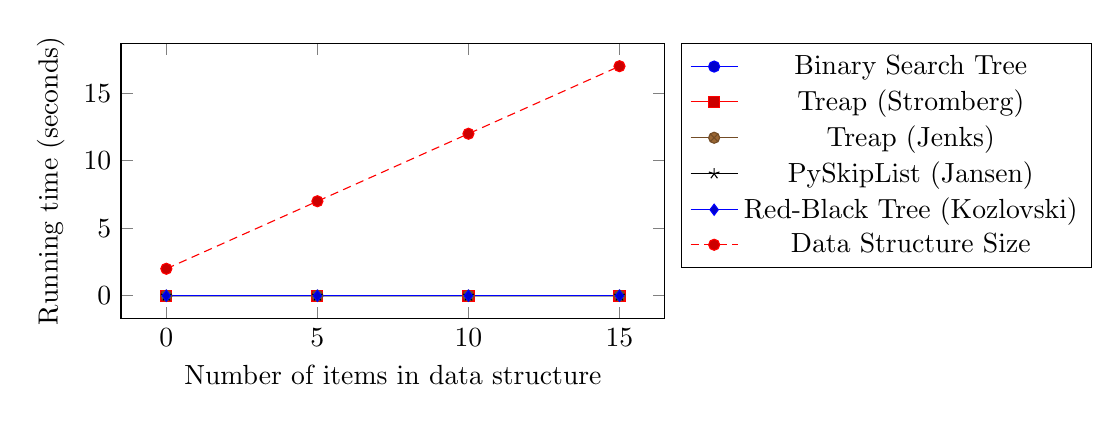
\begin{tikzpicture}
        \begin{axis}[
            xlabel={Number of items in data structure},
            ylabel={Running time (seconds)},
            title={},
            width=0.7\textwidth,
            height=2in,
            legend pos=outer north east
        ]
		\addplot coordinates {
			(0, 3.4133204831857055e-06)
			(5, 3.112145146434072e-06)
			(10, 3.0117533675169095e-06)
			(15, 2.9113615885997465e-06)
		};
		\addplot coordinates {
			(0, 5.119980724778486e-06)
			(5, 5.220372503695649e-06)
			(10, 3.814887598854501e-06)
			(15, 4.116062935606279e-06)
		};
		\addplot coordinates {
			(0, 3.5137122621027236e-06)
			(5, 2.7105780307651317e-06)
			(10, 3.212536925351235e-06)
			(15, 2.7105780307648424e-06)
		};
		\addplot coordinates {
			(0, 1.6464251742424826e-05)
			(5, 1.2950539480321814e-05)
			(10, 1.395445726949431e-05)
			(15, 1.1243879238729179e-05)
		};
		\addplot coordinates {
			(0, 3.212536925351235e-06)
			(5, 3.312928704268398e-06)
			(10, 3.112145146434072e-06)
			(15, 3.6141040410198866e-06)
		};
		\addplot coordinates {
			(0, 2)
			(5, 7)
			(10, 12)
			(15, 17)
		};
        \legend{Binary Search Tree, Treap (Stromberg), Treap (Jenks), PySkipList (Jansen), Red-Black Tree (Kozlovski), Data Structure Size}
        \end{axis}
    \end{tikzpicture}
    \caption{Average of 3 operations, benchmarked every 5, starting at 0.}
\end{figure}